\documentclass[11pt, letterpaper]{article} 

%%%% ----- PACKAGES ---- %%%%

% Fonts & Colors
\usepackage[utf8]{inputenc}
\usepackage[T1]{fontenc}
\usepackage{lmodern}
\usepackage[svgnames,usenames,dvipsnames,x11names,table]{xcolor}
\usepackage{microtype}

% Math 
\usepackage{amsmath,amsthm}
\usepackage{amsfonts,eucal,amssymb,amscd,empheq,bm,mathtools}
\usepackage{mathrsfs}
\usepackage{calc} 

% Tikz & boxes
\usepackage{tikz}
\usepackage[framemethod=tikz]{mdframed}
\usepackage{framed}

% interface for floats (Figures/Tables), allows 'H' option
\usepackage{float}

% expanded footnote package
\usepackage{bigfoot}

% refinements 
\usepackage{setspace}
\usepackage{graphicx}
\usepackage[normalem]{ulem}
\usepackage{fancyhdr}
\usepackage[pdftex]{hyperref}
\usepackage{url}

%\usepackage{amsmath, amsfonts, amsthm}
%\usepackage[svgnames,table]{xcolor}
\usepackage[hang, small, labelfont=bf, up, textfont=it]{caption}
\usepackage{booktabs} 

\usepackage{enumerate}
\usepackage{listings}
\usepackage{marginnote}
\usepackage{mparhack}

\usepackage{longtable}
\usepackage[labelfont=bf,indention=0cm]{caption}
\usepackage{subcaption}

\usepackage{verbatim}
\usepackage[makeroom]{cancel}

\usepackage{geometry}
\usepackage[most]{tcolorbox}
\usepackage{tabularx}

\usepackage{bookmark}
\usepackage[lite]{amsrefs}
\usepackage{arydshln}

\usepackage{booktabs}
\newcounter{lecnum}
\usepackage{nicefrac}
\usepackage{tcolorbox}
\tcbuselibrary{theorems}

\usepackage{enumitem} 
\setlist{noitemsep} 
\usepackage{sectsty} 
\allsectionsfont{\usefont{OT1}{phv}{b}{n}}

\makeatletter
\def\@seccntformat#1{\csname the#1\endcsname.\quad}
\makeatother

\usepackage{geometry}
\geometry{
	top=0.75in,
	bottom=0.75in,
	left=1.5in,
	right=1.5in,
	includehead,
	includefoot,
	%showframe, 
}

\hypersetup{pdftex, colorlinks, citecolor=blue, filecolor=blue, linkcolor=blue, urlcolor=blue}

\pagestyle{fancy}
\PassOptionsToPackage{normalem}{ulem}
\makeindex
\setlength{\headheight}{12pt}


\setlength{\columnsep}{7mm} % Column separation width
\usepackage[T1]{fontenc}
\usepackage[utf8]{inputenc} 
\usepackage{XCharter} 
\usepackage{fancyhdr} 
\pagestyle{fancy} 

\renewcommand{\headrulewidth}{0.0pt} 
\renewcommand{\footrulewidth}{0.0pt}

%\renewcommand{\footnotesize}{\scriptsize}
\setlength{\skip\footins}{10pt}

\usepackage[numbered,framed]{matlab-prettifier}
\lstset{style= Matlab-editor,
    basicstyle = \mlttfamily\footnotesize,
    breaklines=false,
    %backgroundcolor=\color{light-gray},
    numbersep=5pt,
    xleftmargin=.25in,
    xrightmargin=.25in 
} 

%\usepackage[parfill]{parskip}
%\setlength{\parskip}{4pt} 
\setlength{\parindent}{0pt}

% format/layout adjustments
\newcommand{\n}{\vskip 6pt \noindent}
\newcommand{\nn}{\vspace{8mm} \noindent}
\newcommand{\ns}{\vspace{8mm}}

% for adjustwidth environment
\usepackage[strict]{changepage}

% environment derived from framed.sty: see leftbar environment definition
\definecolor{formalshade}{rgb}{0.95,0.95,1}
\definecolor{darkBlue}{RGB}{25,25,112}

\newenvironment{formal}{%
\small
  \def\FrameCommand{%
    \hspace{1pt}%
    {\color{darkBlue}\vrule width 2pt}%
    {\color{formalshade}\vrule width 4pt}%
    \colorbox{formalshade}%
  }%
  \MakeFramed{\advance\hsize-\width\FrameRestore}%
  \noindent\hspace{-4.55pt}% disable indenting first paragraph
  \begin{adjustwidth}{}{7pt}%
  \vspace{-12pt}
  \vspace{2pt}\vspace{2pt}%
}
{%
  \vspace{2pt}\end{adjustwidth}\endMakeFramed%
}

\usepackage{sectsty}
\subsectionfont{\normalfont\itshape}


% Removes the section number from the header when \leftmark is used
\renewcommand{\sectionmark}[1]{\markboth{#1}{}} 

\usepackage{titlesec}
\titleformat{\subsubsection}{}{\thesubsubsection}{1em}{\itshape}



%\nouppercase\leftmark % Add this to one of the lines below if you want a section title in the header/footer

% Headers/ footers
\lhead{}
\chead{} 
\rhead{}

\lfoot{} 
\cfoot{} 
\rfoot{} % Right footer, "Page 1 of 2"

\fancyfoot[C]{\fontsize{9}{12} \selectfont \vspace{12pt} \textit{\footnotesize{\thepage}}}

% Page style for the first page with the title
\fancypagestyle{firstpage}{ 
	\fancyhf{}
	\renewcommand{\footrulewidth}{0pt}
}

%----------------------------------------------------------------------------------------
%	TITLE SECTION
%----------------------------------------------------------------------------------------

\newcommand{\authorstyle}[1]{{\large\usefont{OT1}{phv}{b}{n}\color{DarkRed}#1}} 
\newcommand{\institution}[1]{{\footnotesize\usefont{OT1}{phv}{m}{sl}\color{Black}#1}}
\usepackage{titling} 
\newcommand{\HorRule}{\noindent \color{DarkGoldenrod}\rule{\linewidth}{0pt}} 

\pretitle{
\centering
	\vspace{-5pt} 
	\HorRule\vspace{10pt} 
	\fontsize{24}{28}\usefont{OT1}{phv}{m}{n}\selectfont 
	\color{DarkRed} 
}
\posttitle{
\centering
\par\vskip2pt
} 

\preauthor{} 
\postauthor{ 
	\vspace{0pt} 
	\par\HorRule
	%\vspace{20pt} 
	\vspace{-1cm} 
}


\theoremstyle{break}
\newtheorem{example}{Example}[section]

\mdfdefinestyle{mystyle}{
  hidealllines=true,
  leftline=true,
  innerleftmargin=10pt,
  innerrightmargin=10pt,
  innertopmargin=10pt,
}


\newmdtheoremenv[style=mystyle]{example2}{Example}




\theoremstyle{definition}
\newtheorem{defnn}{Definition}
\newtheorem*{tst*}{}
\newmdtheoremenv[style=mystyle]{defnn2}{Definition}

\newtheorem*{Alg*}{Algorithm}
\newtheorem*{rmk*}{Remark}
\newtheorem*{thm}{Theorem}
\newcommand{\Recall}{\vspace{4mm}\noindent \bd{\ul{Recall}}}
\newcommand{\Note}{\vspace{4mm}\noindent \bd{\ul{Note}}}
\newcommand{\Question}{\vspace{4mm}\noindent \bd{\ul{Question}}}

\newcommand{\Problem}[1]{\vspace{4mm}\noindent {\large\bd{\ul{Problem #1}}}}



		%%%%%%%%%%%%%%%%%%%%%%%%%%%%%%%% DEFINITIONS  %%%%%%%%%%%%%%%%%%%%%%%%%%%%%%%%%%%

\theoremstyle{definition}
\newtheorem{quest}{Question Set:}
\newtheorem{deliv}{Deliverable}



%%%%%%      MATH ENVIRONMENT      %%%%%%%%

% align
\newcommand{\eq}[1]{\begin{align*}#1\end{align*}}

% tags
\newcommand{\tagit}[1]{\tag{\it{#1}}}
\newcommand{\tagitb}[1]{\textcolor{blue}{\tag{\it{#1}}}}



% font
\newcommand{\ul}[1]{\underline{#1}}
\renewcommand{\it}[1]{\textit{#1}}
\newcommand{\bd}[1]{\textbf{#1}}
\newcommand{\bul}[1]{\textbf{\ul{#1}}}
\newcommand{\bit}[1]{\textbf{\textit{#1}}}



% shortcuts for letters, symbols & etc
\def\nhat{\bm{\hat{n}}}

\newcommand{\Z}{{\mathbb{Z}}}
\newcommand{\R}{{\mathbb{R}}}
\newcommand{\N}{{\mathbb{N}}}
\newcommand{\F}{{\mathcal{F}}}
\newcommand{\C}{{\mathcal{C}}}
\newcommand{\W}{{\mathcal{W}}}
\newcommand{\E}{{\mathcal{E}}}
\newcommand{\A}{{\mathcal{A}}}
\newcommand{\X}{{\mathbb{X}}}


% colors
\colorlet{shadecolor}{Red!5}
\colorlet{framecolor}{Red!1}
\definecolor{dkred}{RGB}{165,0,0}

%%%%% BOXED EQUATIONS %%%%%%%
\newcommand*\widefbox[1]{\fbox{\hspace{2em}#1\hspace{2em}}}

% shading
\newenvironment{frshaded}{
 \def\FrameCommand{\fboxrule=\FrameRule\fboxsep=\FrameSep \fcolorbox{framecolor}{shadecolor}}%
 \MakeFramed{\FrameRestore}}%
 {\endMakeFramed}

 \newenvironment{frshaded*}{%
 \def\FrameCommand{\fboxrule=\FrameRule\fboxsep=2\FrameSep \fcolorbox{framecolor}{shadecolor}}%
 \MakeFramed{\advance \hsize - \width \FrameRestore}}%
  {\endMakeFramed}



% horizontal & vertical lines
\newcommand*{\vertbar}{\rule[-1ex]{0.5pt}{2.5ex}}
\newcommand*{\horzbar}{\rule[.5ex]{3ex}{0.5pt}}

%%%%%%      SHORTCUTS     %%%%%%%%
\newcommand{\dt}{{\Delta t}}
\newcommand{\dx}{{\Delta x}}
\newcommand{\idt}{{\frac{1}{\Delta t}}}
\newcommand{\idx}{{\frac{1}{\Delta x}}}
\newcommand{\dtdx}{\frac{\Delta t}{\Delta x}}
\newcommand{\dxdt}{\frac{\Delta x}{\Delta t}}

\newcommand{\Qin}{{Q_{i}^{n} }}
\newcommand{\Qini}{{Q_{i}^{n \+ 1} }}
\newcommand{\Qimi}{{Q_{i}^{n \- 1} }}
\newcommand{\Qinp}[1]{{Q_{i}^{n \+ #1} }}

\newcommand{\qx}{q_{,x}}
\newcommand{\qxx}{q_{,x,x}}
\newcommand{\qt}{q_{,t}}
\newcommand{\qtt}{q_{,t,t}}

\newcommand{\ordii}{\ord( \dx^2)}
\newcommand{\ordiii}{\ord( \dx^3)}

\renewcommand{\uplus}{u^{\+}}
\newcommand{\uminus}{u^{\-}}

\newcommand{\Fii}[2]{\F_{ i \+ \h}^{n \+ \h}}
\newcommand{\Fnn}[2]{\F_{ #1}^{#2}}
\newcommand{\FF}{\Scale[1.4]{\mathscr{F}}}

\newcommand{\sumN}{\sum_{i \= 1}^{N} }
\newcommand{\summ}{\sum_{p \= 1}^{m} }
\newcommand{\suminf}{\sum_{i \= -\infty}^{\infty} }

\newcommand{\ord}{{\mathcal{O}}}
\newcommand{\into}{\rightarrow}

\newcommand{\stari}{\raisebox{.2\height}{\scalebox{0.9}{\ensuremath{\hspace{0.25mm} \star}}}}


\newcommand{\lp}{\lambda^{(p)}}

%% SUPERSCRIPTS
\newcommand{\soln}{\it{sol}\textsuperscript{\ul{\it{n}}}}
\newcommand{\Soln}{\it{Sol}\textsuperscript{\ul{\it{n}}}}
\newcommand{\eqn}{\it{eq}\textsuperscript{\ul{\it{n}}}}
\newcommand{\Eqn}{\it{Eq}\textsuperscript{\ul{\it{n}}}}

\newcommand{\st}{\textsuperscript{\ul{\it{st}}} }
\newcommand{\nd}{\textsuperscript{\ul{\it{nd}}} }

% create a matrix: use &, \\ as normal
\newcommand{\mtx}[1]{\left(\begin{matrix}#1\end{matrix}\right)}


%%%%% EQUATIONS  %%%%%%

\newcommand{\burgers}{\eq{  q_{,t} + \Big( \h q^2 \Big)_{,x} = 0 }} 			% Burger's Eqn






%%%%% GRAPHICS %%%%%
\newcommand{\gfxi}[1]{
\vspace{3mm}
  \begin{center}
    \begin{figure}[h!]
    \includegraphics[height=45mm]{#1}
    \end{figure}
  \end{center}
}

\newcommand{\gfxii}[2]{
\vspace{3mm}
  \begin{center}
    \begin{figure}[h!]
    \includegraphics[height=#1mm]{#2}
    \end{figure}
  \end{center}
}

% figure + equation/text, side by side
\newcommand{\gfxss}[2]{
\vspace{3mm}
\noindent\begin{minipage}{.45\textwidth}
 	\centering
   		\includegraphics[height=45mm]{#1}
  		\label{fig:figure}
\end{minipage}
\begin{minipage}{.45\textwidth}
#2
\end{minipage}
}

 
\graphicspath{{./gfx/}}

\title{ \textsc{Prelab Exercise 1: \\ Linear Heat Conduction} \\ {\large  \color{darkgray} ME 436 Heat Transfer}}

\begin{document}
\date{}
\maketitle
\thispagestyle{firstpage} 

\section*{Introduction}

The objective of this experiment is to explore \it{Fourier’s Law} for linear conduction by studying steady-state heat transfer through various materials. Completion of this assignment will provide you with the necessary tools to properly study and explore your collected lab data.

\section*{Prerequisites}
Before attempting this pre-lab assignment, it is imperative that you have:
{\small
\begin{itemize}
    \item Reviewed the \bit{textbook sections:} 2.1, 2.2 \& 3.1-3.1.4,
    \item Reviewed the \bit{experiment procedures}, 
    \item Watched the \bit{pre-lab videos} on Blackboard (Bb), and
    \item Completed the \bit{pre-lab quiz} on Bb.
\end{itemize}
}

\section*{Getting Started}
First, be sure to download the starter code from Blackboard (Bb), and \textit{extract} (unzip) its contents to the directory in which you wish to complete the exercise\footnote{\textit{Note: when using the Heat Transfer Lab computers, you \ul{must} extract your code to the local hard drive: \texttt{C:/temp/}, NOT to the server (ie., Desktop, Group Folder, \&, etc.)}}. Before attempting, make sure that you have completed all of the \textit{prerequisites} below.

\subsection*{Files included in this exercise:}
Once you have unzipped the contents of the starter package, you should see the following files:

\begin{itemize}
\renewcommand\labelitemi{-- }
   \item \texttt{ex1.m}
    \item \texttt{/lib}
   \item \texttt{/data}
\renewcommand\labelitemi{[$\star$]}
    \item \texttt{plotData.m}
    \item \texttt{calc\_ks.m}
    \item \texttt{fouriers\_law.m} 
    \item \texttt{calc\_contact\_res.m} 
\end{itemize}

\noindent
$\star$ indicates files that you will need to complete.\\

\n
Throughout this exercise, you will be using the script \texttt{ex1.m}, but will not be required to make any major modifications to it. You are only required to modify the functions \textit{(often only 1-2 lines of code)} in the files specified above. Your submission will consist of a compilation (via word processor) of \textit{`deliverables'}, specified throughout this document. Instructions for each deliverable will be highlighted in a blue box, similar to the following: 
\setcounter{deliv}{-1}
\begin{formal}
    \begin{deliv} \bit{Sample}s
    
Follow the instructions in this blue box.
    \end{deliv}
\end{formal}


\setcounter{section}{-1}
\section{Warm-Up \& System Check}

Before starting, it's often a good idea understand the data by first visualizing it. This section will walk you through the essentials of doing so. \textit{If you have any difficulties getting started, be sure to ask your TA for assistance.} \n

\noindent
First, open the Matlab script \texttt{ex1.m} and read through the instructions. The section immediately following, clears the workspace and initializes our paths and raw data variable. Next, we get to a section titled \textit{`Load Data'}. Here, we load a sample dataset from a text file and store it into the variable \texttt{M}:
\n
\begin{lstlisting}[numbers=none]
% load tab separated data
M = load('data.txt'); 
\end{lstlisting}
\n
Now, we have a matrix $M$ of size $93 \times 11$ ($rows \times columns$), or $M \in \mathbb{R}^{93 \times 11}$. The columns in $M$ correspond to:
\\
{\small
\begin{center}\renewcommand{\arraystretch}{1.5}
\begin{tabular}{|c | c | c | c | c | c | c |}
\hline
\rowcolor{light-gray}
    1 & 2 & 3 & \dots & 9 & 10 & 11 \\ 
    \hline
   \cellcolor{green!10} $time (s)$ & \cellcolor{red!10}$TC_1$ & \cellcolor{red!10}$TC_2$ & \cellcolor{red!10}$\dots$ & \cellcolor{red!10}$TC_8$ & \cellcolor{orange!10}$Voltage, V$ & \cellcolor{orange!10}$Current, A$ \\ 
\hline
\end{tabular}
\end{center}
}

In which $TC_n$ refers to the thermocouple number, read in degrees Celsius. Next, you will see a line that looks similar to the following:
\n
\begin{lstlisting}[numbers=none]
% COMMENT ME OUT!!
break_msg; dbstack; return;
\end{lstlisting}

\n
This is what we refer to as a \texttt{return} command. You will need to \textit{comment out} this line (place a \% out front) in order to continue. 

\n
Next, let's separate out this data into more meaningful variables.\footnote{\textit{Note: if you are not familiar with the syntax, check out: \href{https://www.mathworks.com/company/newsletters/articles/matrix-indexing-in-matlab.html}{Matrix indexing in Matlab}  }} 
\n
\begin{lstlisting}[numbers=none]
t = M(:,1);         % get time vector, [s]
dat = M(:,2:9);     % get temps, [C]
V = M(:,10);        % Voltage, [V]
I = M(:,11);        % Current, [A]
\end{lstlisting}

\n
Then we simply plot temperature with time:
\n
\begin{minipage}{\linewidth}
\begin{lstlisting}[numbers=none]
figure;         % open new figure
h = plot(dat);  % plot the data
set(h, 'LineStyle', '-', 'LineWidth', 2)   % make sure the lines are readable
\end{lstlisting}
\end{minipage}

\n
\begin{minipage}{\linewidth}
\begin{lstlisting}[numbers=none]
% don't forget to add labels!!
xlabel('Time [s]');
ylabel('Temperature [C]');
title('Transient Data, T/C','FontSize',16);
grid on
\end{lstlisting}
\end{minipage}

\n
Now, if everything was done correctly, you should get something similar to Fig.~\ref{fig1} below.

\begin{figure}[H]
    \begin{center}
        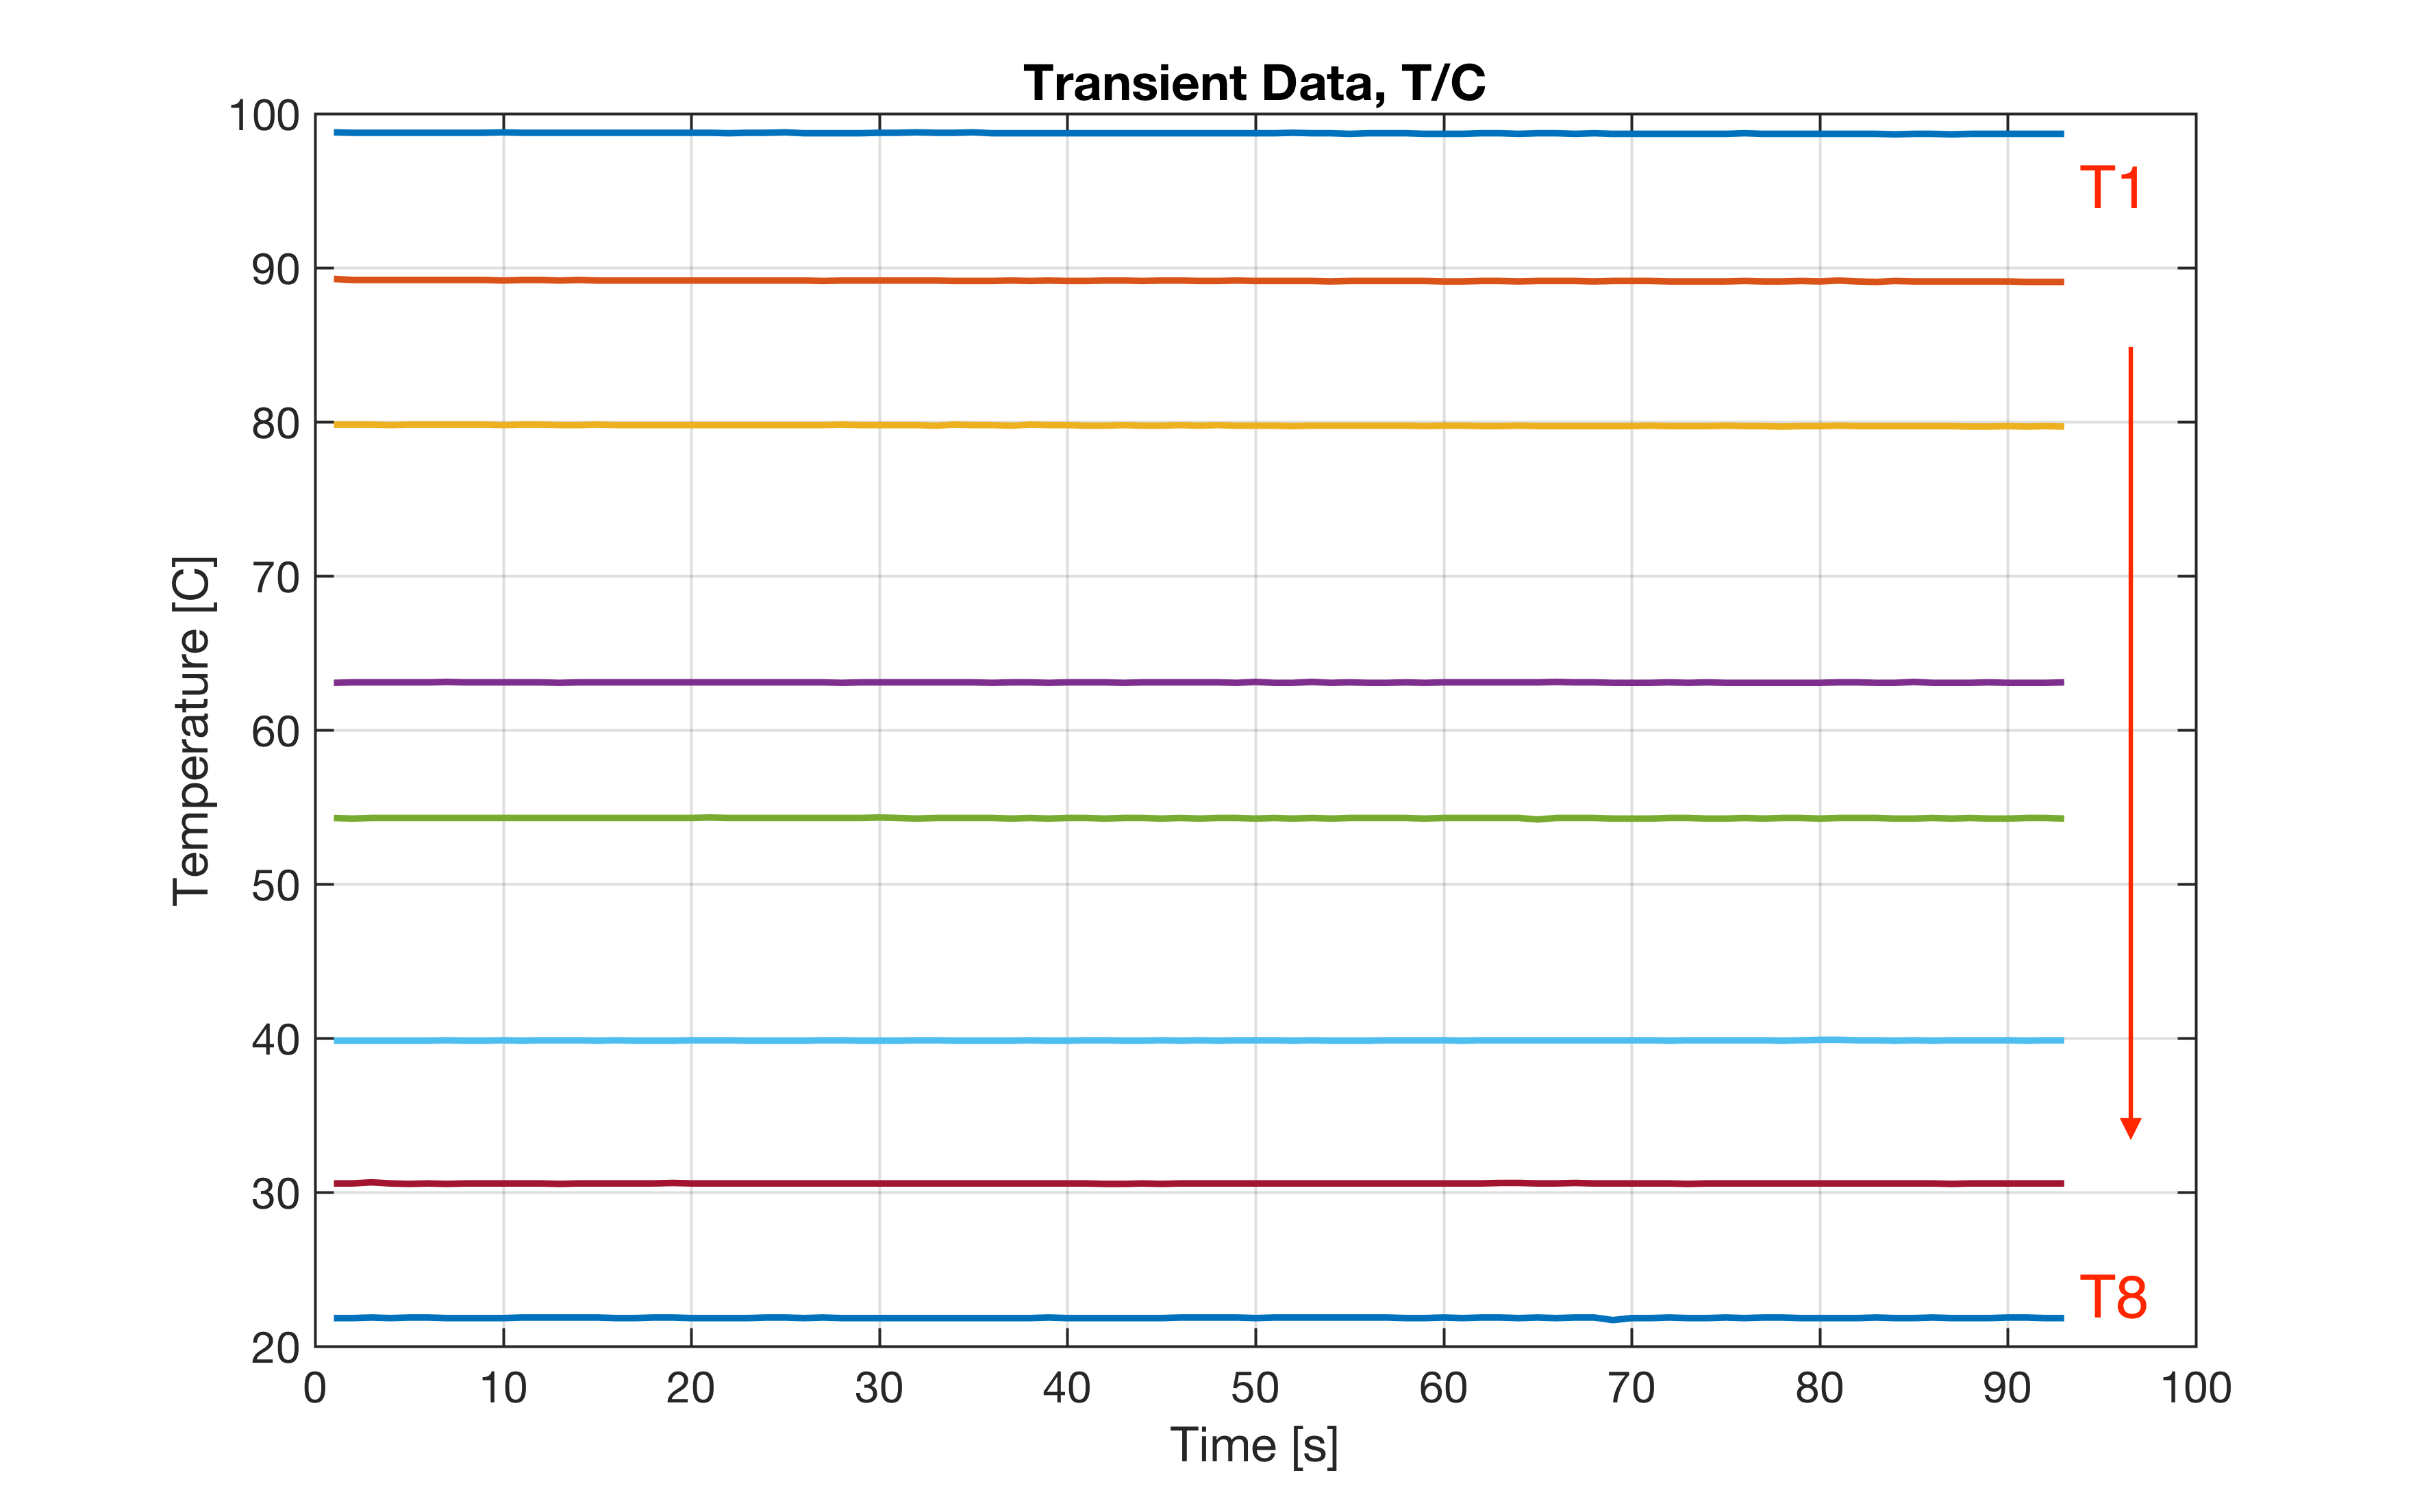
\includegraphics[width=125mm]{gfx/fig1.png}
    \caption{Transient temperature data}\label{fig1}
    \end{center}
\end{figure}

A few quick questions to ask:

\begin{formal}
\begin{quest} \bit{Sanity Check.}
\begin{itemize}
    \item Does your plot match Fig.~\ref{fig1} above? 
    \item \it{Are you using the correct version of \texttt{MATLAB}?} 
    \item Is all of our data at steady-state?
\end{itemize}
\end{quest}
\end{formal}
\begin{center}
\begin{tcolorbox}[enhanced, width=14cm, top=-2mm, colback=red!5, colframe=black!50!white, boxrule=0.25pt, boxsep=2mm]
\n
{\small
\bit{Checkpoint} - If you had any difficulties obtaining Fig.~\ref{fig1}, \bul{stop here} and contact your Lab Instructor. You may run into more troubles ahead.
}
\end{tcolorbox}

\end{center}

When you're ready to continue, comment out the following line:

\n
\begin{lstlisting}[numbers=none]
% remove break
break_msg; dbstack; return;
\end{lstlisting}

\n
\hrule

\section{Plot Steady-State Data}

Now, let's plot the spatial temperature distribution. To do this, we simply average the transient data. This is easily done in \texttt{MATLAB} by the $mean( )$ command:

\begin{lstlisting}[numbers=none]
% take an average of the last (~20) points 
N = 20;
Tm = mean(dat(end-N:end,:));      % [C]
Vm = mean(V(end-N:end));          % [V]
Im = mean(I(end-N:end));          % [A]
\end{lstlisting}

Next, we call a \texttt{plotData.m} function to plot our data. As-it-is, this plot function \textit{\ul{is incorrect}} and will not run properly. Therefore, you will need to open \texttt{plotData.m} and adjust code accordingly in order for it to run properly. The sections that you will need to complete are outlined:

\n
\begin{lstlisting}[numbers=none]
% plot first three T/Cs
plot(x(2:4),y(1:3),'ko-','MarkerSize', 8);

% plot middle two T/Cs
% ====================== YOUR CODE HERE ======================

% plot last three T/Cs
% ====================== YOUR CODE HERE ======================


% set labels & axis limits
% ====================== YOUR CODE HERE ======================
xlabel('');
ylabel('');
\end{lstlisting}

\begin{itemize}
    \item \textit{Note: Pay close attention to the instructions.}
\end{itemize}

When you're finished, you must \bit{go back} to \texttt{ex0.m} before you can press \texttt{Run}. If you attempt to run the function \texttt{plotData.m}, you will receive an error. If your adjustments were correct, and \texttt{ex0.m} was properly executed, you should obtain Fig.~\ref{fig2}.



\begin{figure}[H]
    \begin{center}
        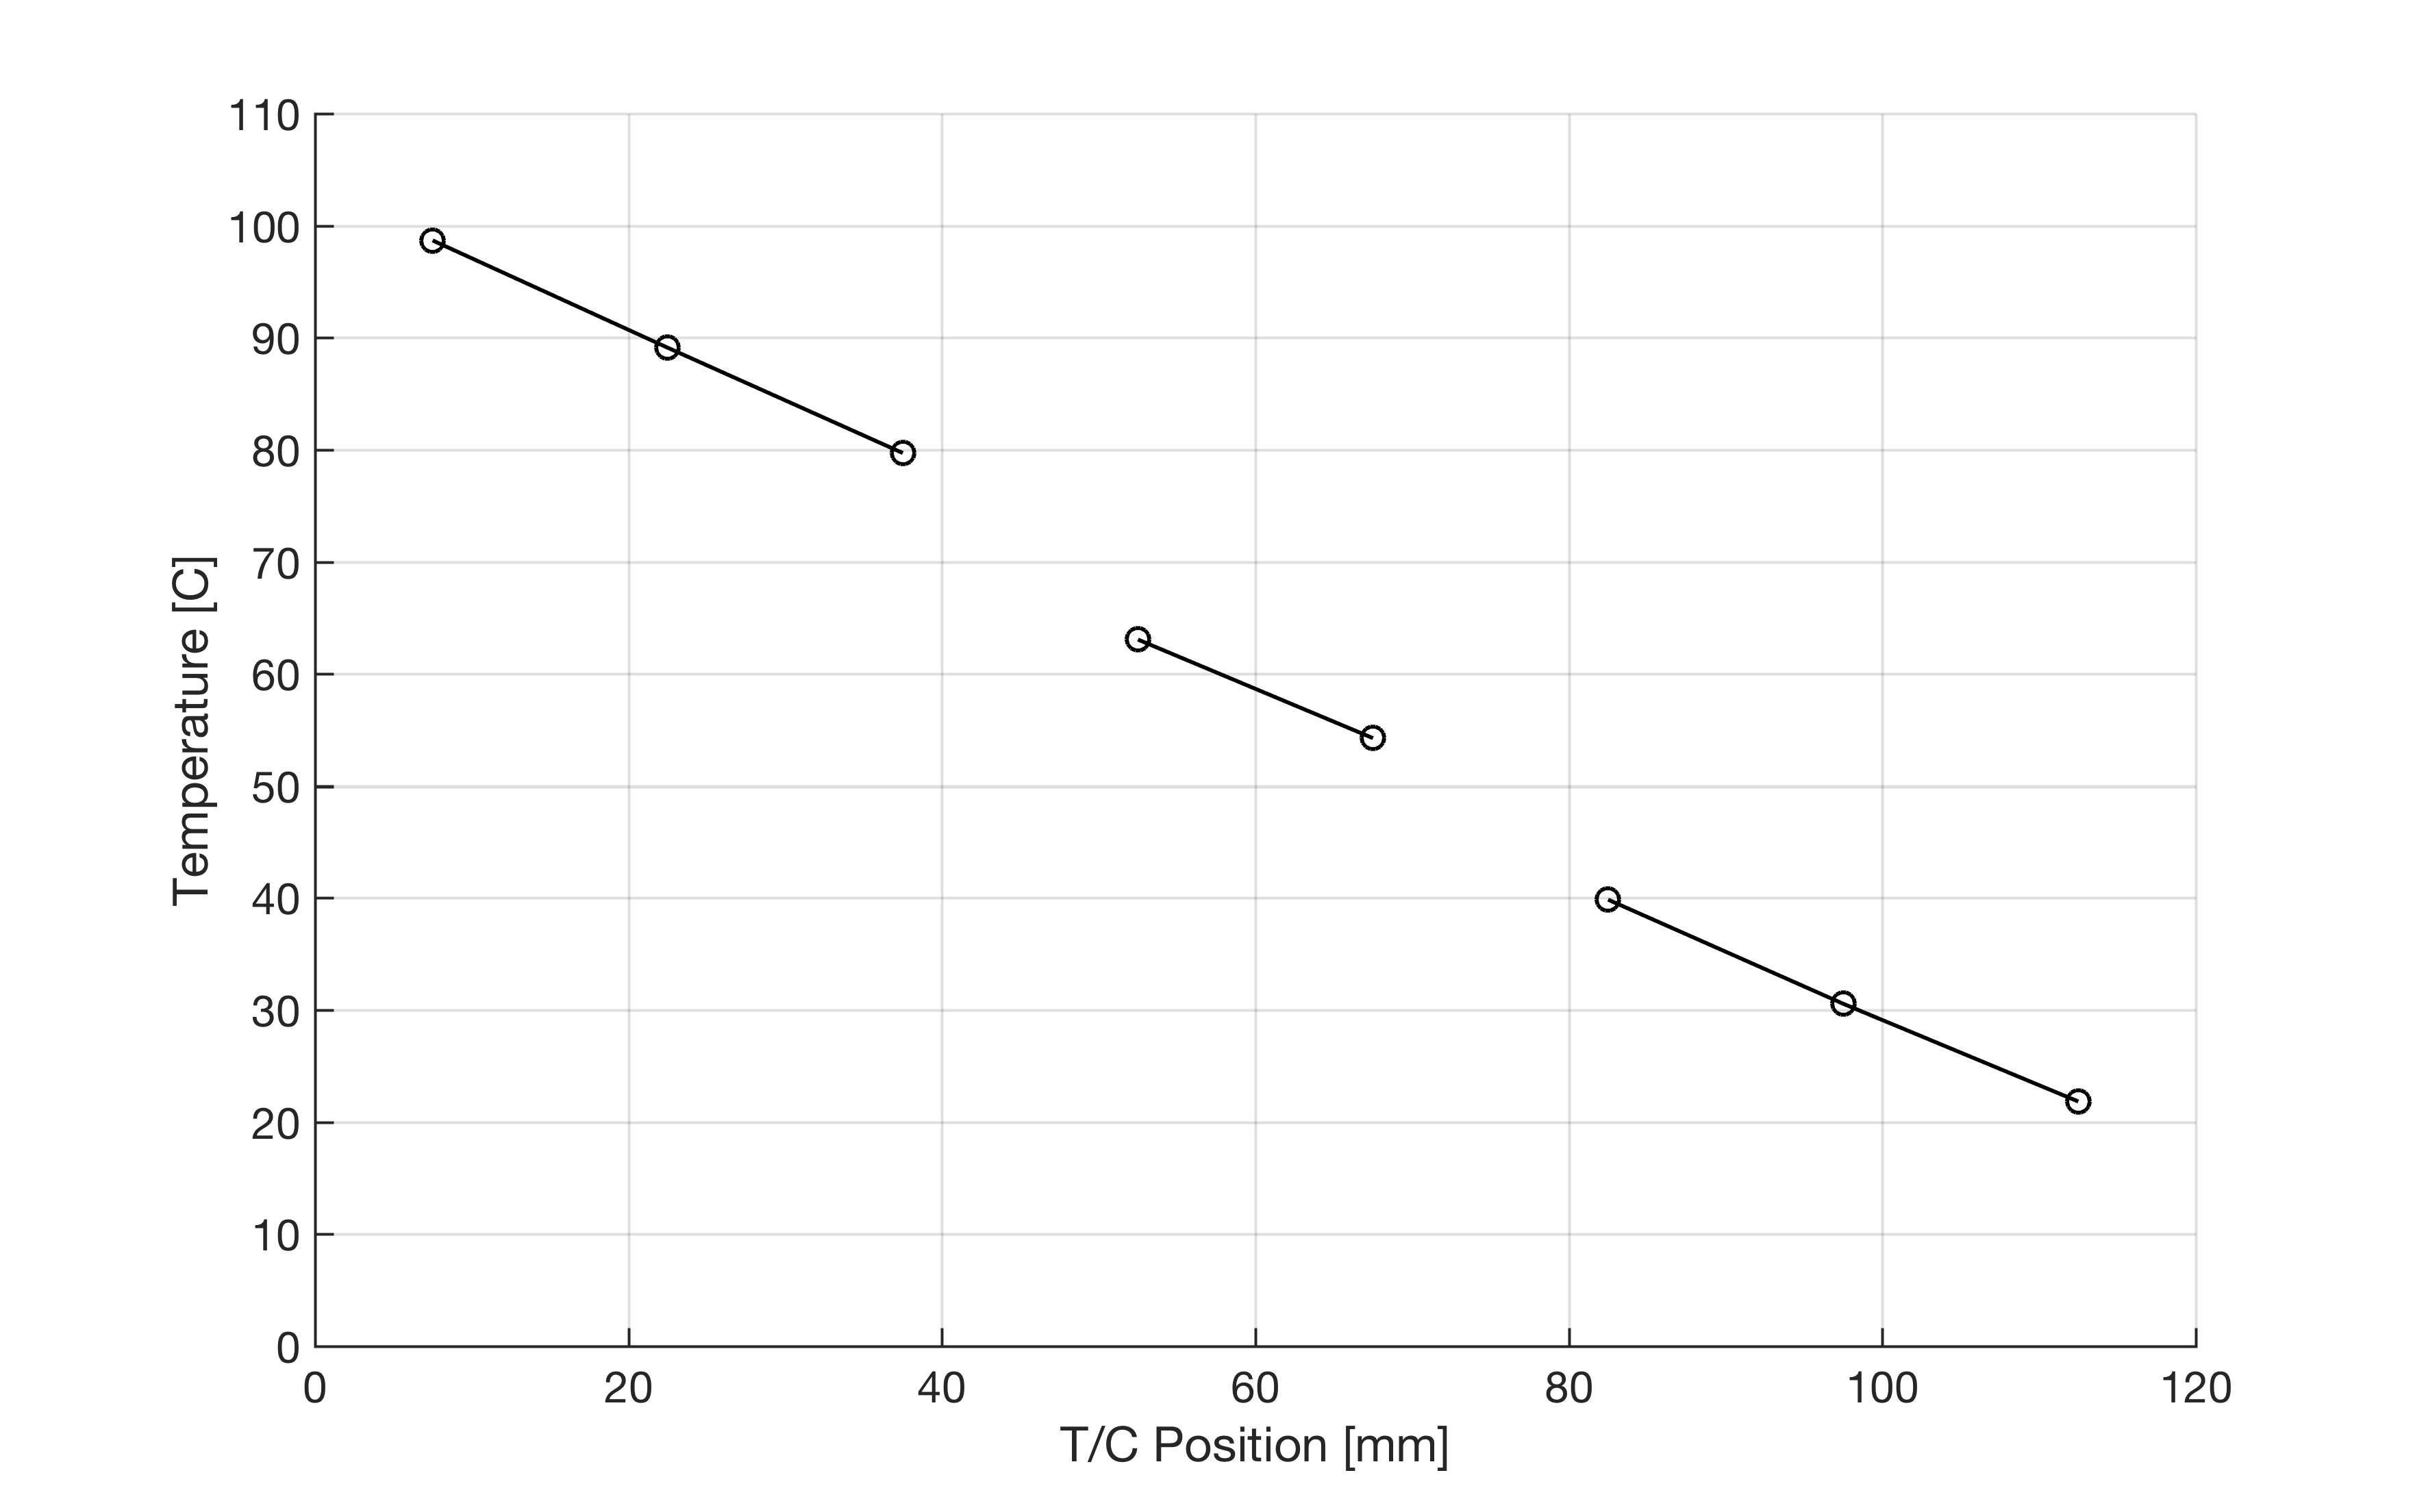
\includegraphics[width=125mm]{gfx/fig2.png}
    \caption{Transient temperature data}\label{fig2}
    \end{center}
\end{figure}

Then, if everything was done correctly in part 1a, you should arrive at a figure that resembles Fig.~\ref{fig3} below.

\begin{figure}[H]
    \begin{center}
        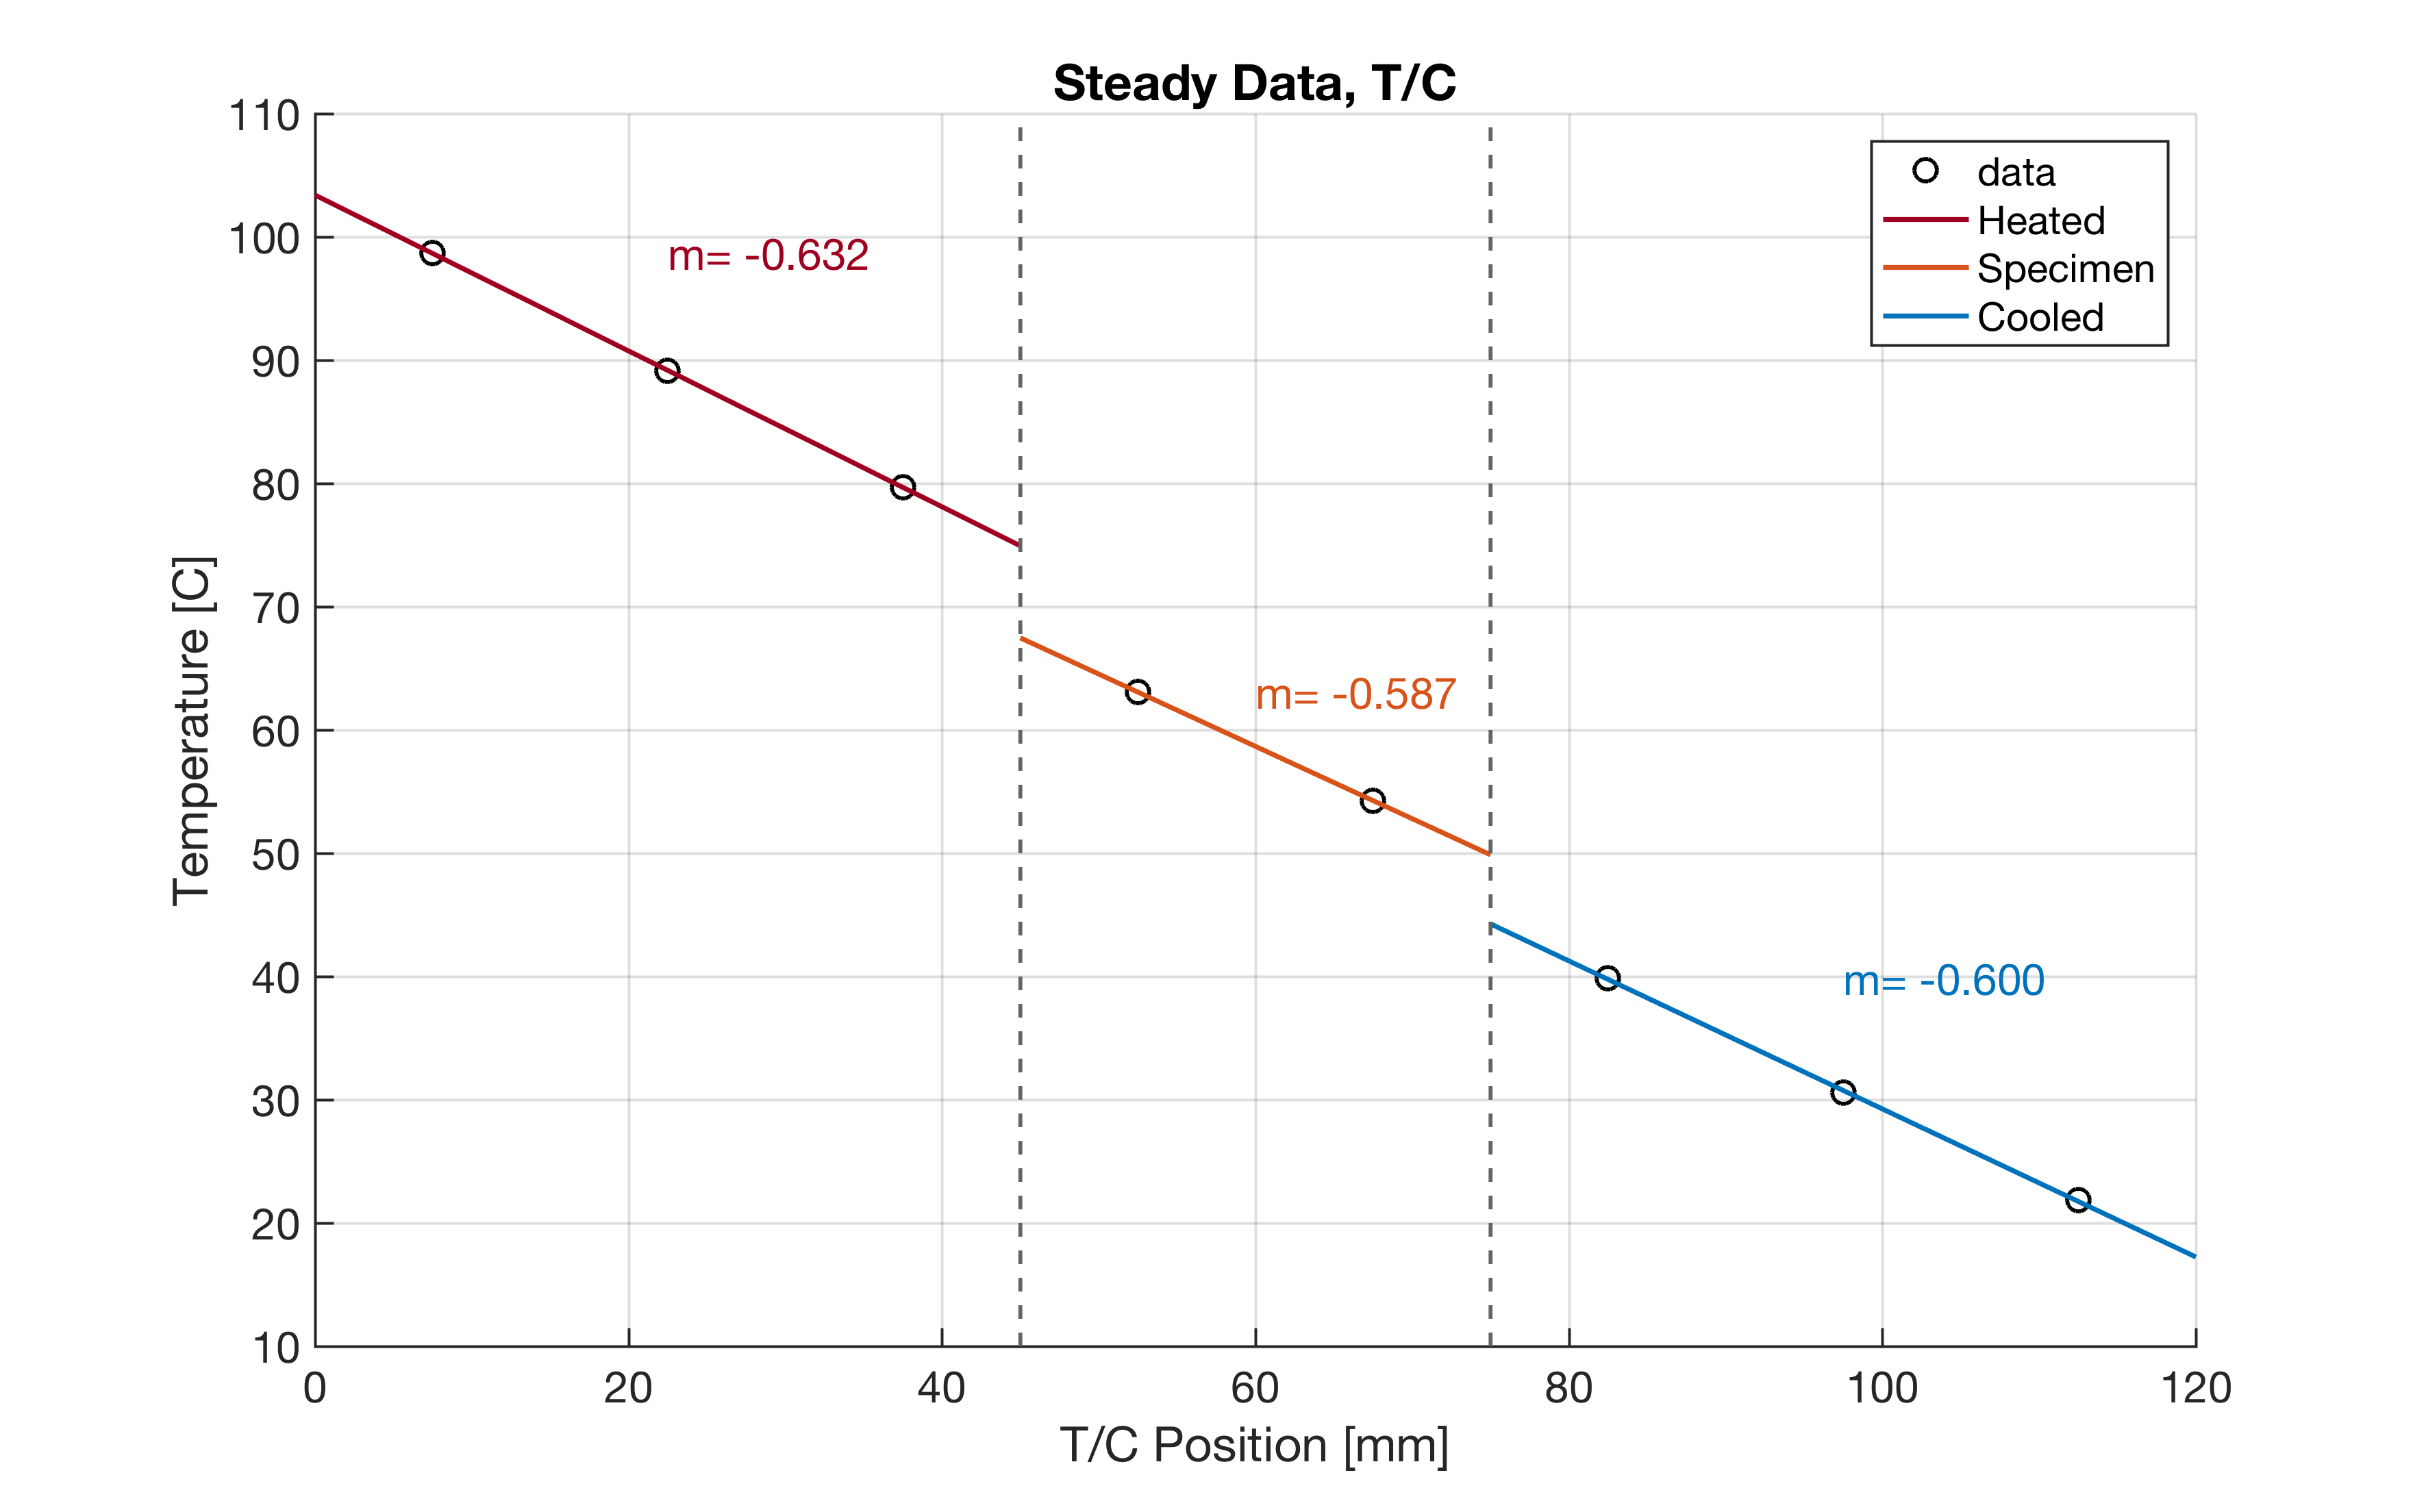
\includegraphics[width=125mm]{gfx/fig3.png}
    \caption{Steady-state T/C data}\label{fig3}
    \end{center}
\end{figure}

Here, we have added regression lines that extend slightly beyond their representative data points --- until they reach a midpoint.  This vertical intersection line dividing the two regression lines, is the \textit{theoretical} point of contact between the two sections. Since we physically can't place a thermocouple at the very edge of each material, these \textit{extrapolated} temperature values are the best we can do. We'll revisit these values when we discuss the contact resistance.

\begin{formal}
    \begin{deliv} \bit{Steady-state T/C plot} (Fig.~\ref{fig3} above) 
    
   Export your figure to an image: \texttt{File >> Export Setup >> Export}, and include it in your submission.
    \end{deliv}
\end{formal}

\n
\hrule
\section{Calculate Sample Thermal Conductivity, $k_s$}

In this exercise, you will calculate the thermal conductivity, $k_s$, of the unknown specimen. This computation is only made possible by one critical assumption: \it{we can safely assume that a \ul{constant heat flux} passes through the entire linear conduction apparatus.} Let's quickly revisit how this is possible.

\subsection{Background}
Assume that we have a generic plane-wall, like that shown to the right. Recall from your lecture notes and p113 of the textbook, \it{\ul{one form} of the heat equation} may be written as:
\eq{
\frac{d}{dx} \Big( k \frac{dT}{dx} \Big) = 0 \tag{\it{Heat Equation}}
}
\begin{minipage}[c]{0.50\textwidth}
{\small
Rewriting:
\eq{ 
k \frac{d^2 T}{dx^2} = 0
}
Integrating twice, boundary conditions:
\begin{align}
    T(x) &= (T_2 - T_1) \frac{x}{L} + T_1
\end{align}
with slope:
\eq{
dT/dx = \frac{(T_2 - T_1)}{L}
}
}
\end{minipage}  \hfill
\begin{minipage}[c]{0.50\linewidth}
\hspace{0mm}
\vspace{-2ex}
    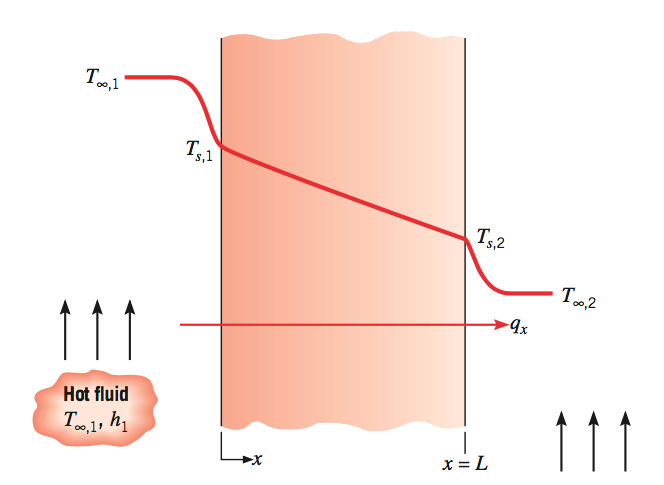
\includegraphics[width=70mm]{gfx/fig4.png}
\vspace{2pt}
\captionof{figure}{1D Schematic}
\end{minipage}

Plugging into Fourier's Law:

\eq{
q_x &= -k A \frac{dT}{dx} \\
& = \frac{k A}{L} ( T_1 - T_2)
}

Finally, the \it{heat flux} is
\begin{align}
    q_x^{\prime\prime} = \frac{k}{L} (T_1 - T_2)
\end{align}

From Eqns. (1) \& (2) we've shown that the temperature profile is \bit{linear} and the heat flux is \bit{constant}, independent of $x$. 

\n
Now, consider the simple composite wall below. Since the heat flux is constant throughout, we can say:






\begin{minipage}[c]{0.50\textwidth}
{\small
\begin{center}
\begin{tcolorbox}[enhanced, width=5cm, top=-4mm, colback=red!5, colframe=black!50!white, boxrule=0.5pt, boxsep=1.5mm, bottom=1mm]
\eq{
q^{\prime\prime}_1 &= q_2^{\prime\prime} \\
- k_1 \Big( \frac{dT}{dx} \Big)_1 &= - k_2 \Big( \frac{dT}{dx} \Big)_2
}
\end{tcolorbox}
\end{center}
}
\end{minipage}  \hfill
\begin{minipage}[c]{0.50\linewidth}
\hspace{-5mm}
\vspace{-2ex}
    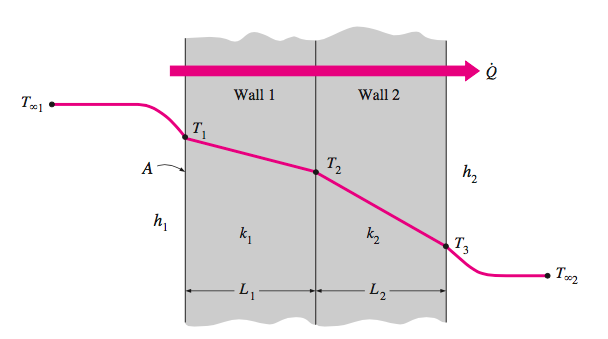
\includegraphics[width=80mm]{gfx/fig5.png}\label{fig5}
\vspace{2pt}
\captionof{figure}{Composite wall}
\end{minipage}

Now, using this information, derive an equation for the unknown $k_s$, before moving on to the next section.

\subsection{Implementation}

Next, we'll prepare a \texttt{MATLAB} function to solve for $k_s$. To do this, open the file named \texttt{calc\_ks.m} and insert the $k_s$ equation that you just derived. You will notice that the derivative terms have already been supplied.

\begin{formal}
    \begin{deliv} \bit{(\ $k_s$\ )} 
    If done correctly, your estimated $k_s$ value will be printed to the \texttt{MATLAB} console. Report your results (including units) and provide 1-2 sentences discussing whether your solution is reasonable or not.
    \end{deliv}
\end{formal}


\section{Calculate Heat Rate}

For this exercise, we calculate the heat rate, $q [W]$, for each section of the experiment apparatus. To do so, open up \texttt{fouriers\_law.m} and insert the appropriate form of Fourier's Law:

\eq{
q_x = -k A \frac{dT}{dx}.  \tag{Fourier's Law}
}

Here, we are looking for the \it{heat rate}, not \it{heat flux} - so be careful with units. If your calculations were performed correctly, your \texttt{MATLAB} console should read:

\begin{lstlisting}[numbers=none]
PART 3: Calculate Heat Rate: 

q[W]: 

     Pin      qh       qs       qc  
    _____    _____    _____    _____
    40.74    37.56    37.56    35.66
 
\end{lstlisting}
In which all units are in Watts $[W]$.

\begin{formal}
    \begin{deliv} \bit{Heat Rate:} 
    Paste your \texttt{MATLAB} console output for this section into your report. Provide 1-2 sentences detailing differences and/or potential loss mechanisms between the $P_{in}$ and your calculated values.
    \end{deliv}
\end{formal}


\section{Calculate Contact Resistance}

Open \texttt{calc\_contact\_res.m} and provide the necessary expressions (see text or lecture notes) for the contact resistance. Your values, if correct, should be on the order of $\approx $ \SI{5e-5}{(m^2 C / W)}.
Next, revisit your Fig.~\ref{fig3} produced above. Are these sharp discontinuities between materials realistic? Consider what factors may play a role in creating these `jumps' and what could be used to minimize them.
\begin{figure}[H]
    \begin{center}
        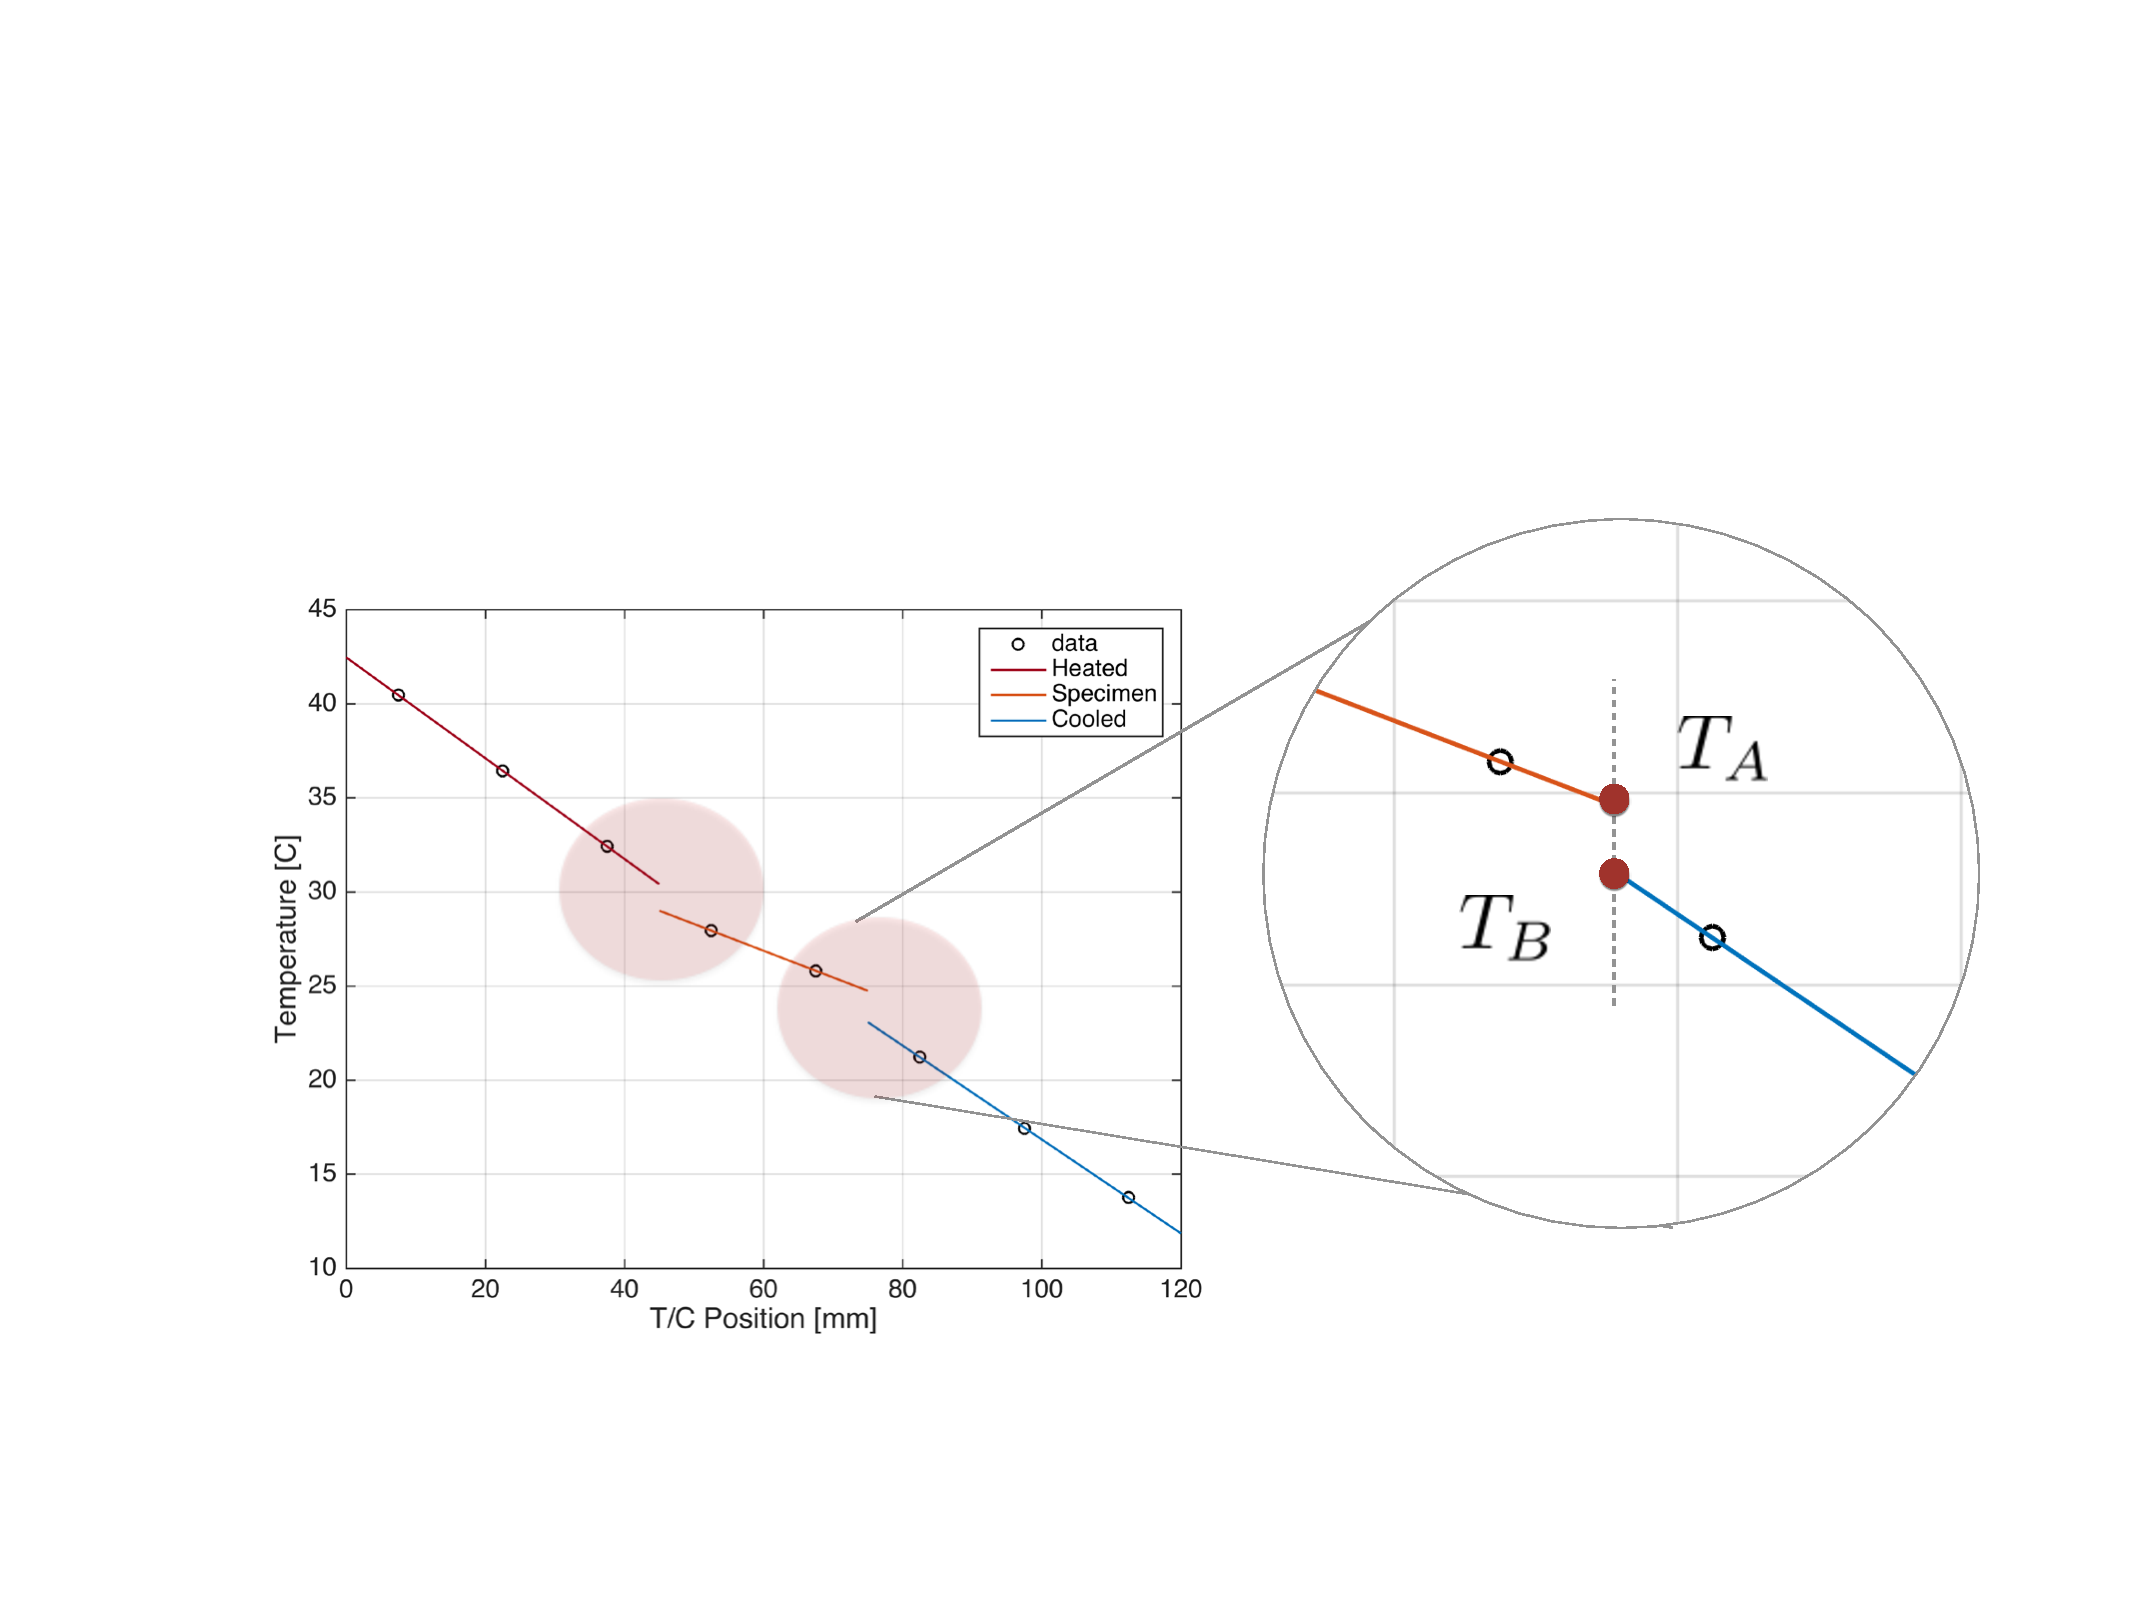
\includegraphics[width=125mm]{gfx/fig6.pdf}
    \caption{Transient temperature data}\label{fig6}
    \end{center}
\end{figure}
\begin{formal}
    \begin{deliv} \bit{Contact Resistance} 
    Paste your \texttt{MATLAB} console output for this section into your report. Provide 1-2 sentences detailing differences and/or potential loss mechanisms between $P_{in}$ and your calculated values.
    \end{deliv}
\end{formal}


\section{Submission}

Compile the above deliverables (blue boxes) into a single document. Be sure to include your name and section number. This assignment will be due when you arrive to class.

\end{document}
